\documentclass[10pt]{article}
\usepackage[margin=0.9in]{geometry}
\usepackage[T1]{fontenc}
\usepackage{lmodern}
\usepackage{amsmath,amssymb,bm}
\usepackage{graphicx,booktabs,array,longtable}
\usepackage{siunitx}
\usepackage{tikz}
\usetikzlibrary{arrows.meta,calc,decorations.pathmorphing,patterns}
\usepackage{xcolor}
\usepackage[hidelinks]{hyperref}
\usepackage{caption}
\captionsetup{font=small}
\definecolor{accent}{HTML}{1F5FA8}
\definecolor{warn}{HTML}{C2410C}
\newcommand{\sgn}{\operatorname{sgn}}
\newcommand{\keybox}[1]{\par\smallskip\noindent\fcolorbox{accent}{accent!6}{\parbox{\dimexpr\linewidth-2\fboxsep-2\fboxrule}{#1}}\par\smallskip}

\title{\textbf{The Falling Inverted Pendulum}\\[2pt]
\large Single arm on a fixed pivot, released from rest, with inertia and friction}
\author{ENGT 480 Pendulum team (Ryan Barney) \quad\textperiodcentered\quad prepared with Claude}
\date{2026-11-20}

\begin{document}
\maketitle

\begin{abstract}
\noindent One rigid arm turns on a fixed, horizontal pivot (the cart is locked or absent). It is held at some angle $\theta_0$ from straight up and let go. This note gives the forward and inverse kinematics, derives the equation of motion with the Lagrangian (including the moment of inertia, viscous friction and Coulomb friction), explains why no exact formula $\theta(t)$ exists once friction is present, gives every closed form that \emph{does} exist (frictionless elliptic solution, small-angle solutions near the top and the bottom), and shows how to solve the full model numerically. Worked numbers use the team's V2 arm~1. A Python solver and an interactive auto-solving calculator come with it.
\end{abstract}

\tableofcontents
\newpage

%=====================================================================
\section{Set-up and sign convention}
%=====================================================================

\begin{figure}[h]
\centering
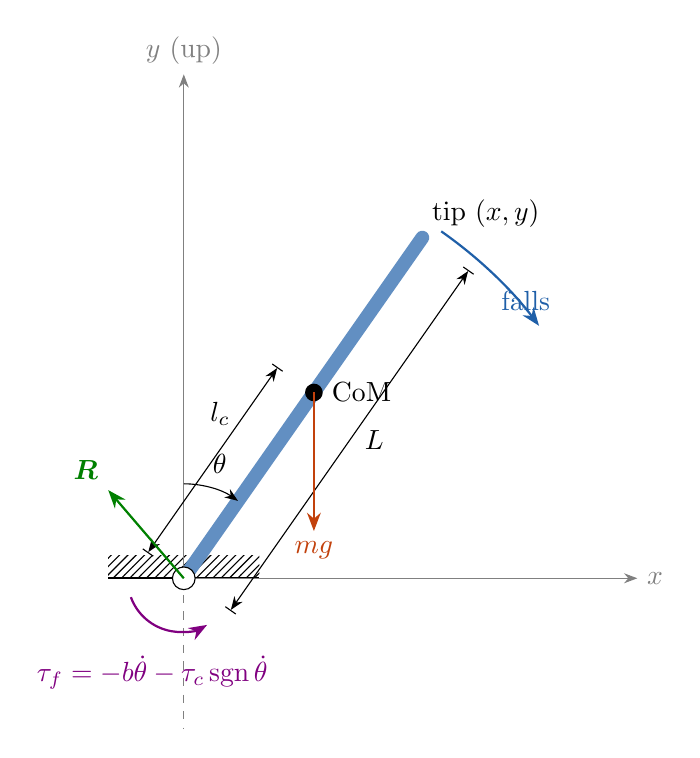
\begin{tikzpicture}[scale=1.6,>=Stealth]
  % pivot support
  \fill[pattern=north east lines] (-0.6,0) rectangle (0.6,0.18);
  \draw[thick] (-0.6,0)--(0.6,0);
  % axes
  \draw[->,gray] (0,0)--(0,4.0) node[above]{$y$ (up)};
  \draw[->,gray] (0,0)--(3.6,0) node[right]{$x$};
  \draw[dashed,gray] (0,0)--(0,-1.2);
  % arm at 35 deg from vertical
  \def\th{35}
  \coordinate (O) at (0,0);
  \coordinate (C) at ({1.8*sin(\th)},{1.8*cos(\th)});
  \coordinate (T) at ({3.3*sin(\th)},{3.3*cos(\th)});
  \draw[line width=5pt,accent!70,line cap=round] (O)--(T);
  \fill[white] (O) circle (0.09); \draw (O) circle (0.09);
  \fill (C) circle (0.07);
  \node[right=3pt] at (C) {CoM};
  \node[above right] at (T) {tip $(x,y)$};
  % theta arc
  \draw[->] (0,0.75) arc (90:{90-\th}:0.75);
  \node at ({0.95*sin(\th/2)},{0.95*cos(\th/2)}) {$\theta$};
  % lc and L
  \draw[|<->|,thin] ($(O)+({-0.35*cos(\th)},{0.35*sin(\th)})$) -- ($(C)+({-0.35*cos(\th)},{0.35*sin(\th)})$) node[pos=0.75,left=2pt]{$l_c$};
  \draw[|<->|,thin] ($(O)+({0.45*cos(\th)},{-0.45*sin(\th)})$) -- ($(T)+({0.45*cos(\th)},{-0.45*sin(\th)})$) node[midway,right=2pt]{$L$};
  % gravity
  \draw[->,thick,warn] (C)--++(0,-1.1) node[below]{$mg$};
  % pivot reaction
  \draw[->,thick,green!50!black] (O)--++(-0.6,0.7) node[above left]{$\bm R$};
  % friction torque
  \draw[->,thick,violet] (-0.42,-0.15) arc (200:300:0.42);
  \node[violet] at (-0.25,-0.75) {$\tau_f=-b\dot\theta-\tau_c\sgn\dot\theta$};
  % motion arrow
  \draw[->,thick,accent] ($(T)+(0.15,0.05)$) arc ({90-\th}:{90-\th-18}:3.45);
  \node[accent,right] at ($(T)+(0.55,-0.5)$) {falls};
\end{tikzpicture}
\caption{Free-body diagram. $\theta$ is measured from straight \emph{up}, positive clockwise (the tip moves toward $+x$). $\theta=0$ is upright, $\pm90^\circ$ is horizontal, $180^\circ$ is hanging. Gravity acts at the centre of mass; the pivot pushes with force $\bm R$ and resists rotation with a friction torque $\tau_f$.}
\label{fig:fbd}
\end{figure}

\noindent Assumptions: rigid arm, planar motion, pivot does not move, air drag is lumped into $b$. The angle is \emph{not} wrapped: after passing the bottom it keeps growing ($270^\circ$ is horizontal on the other side, $360^\circ$ is upright again).

%=====================================================================
\section{Variable key}
%=====================================================================
\begin{center}
\renewcommand{\arraystretch}{1.15}
\begin{longtable}{>{$}l<{$} p{6.8cm} l l}
\toprule
\textrm{Symbol} & Meaning & Unit & V2 arm 1 value\\
\midrule
\endhead
\theta & arm angle from straight up, clockwise positive & rad & \\
\theta_0 & release angle (arm let go at rest) & rad & example $10^\circ$\\
\dot\theta,\ \ddot\theta & angular velocity, angular acceleration & rad/s, rad/s$^2$ & \\
t & time since release & s & \\
m & mass of the arm (everything that turns) & kg & 0.0981\\
L & pivot to tip (the point you track) & m & 0.200\\
l_c & pivot to centre of mass & m & 0.1478\\
s & pivot to any chosen point on the arm & m & \\
I & moment of inertia \emph{about the pivot} & kg\,m$^2$ & $2.484\times10^{-3}$\\
I_{cm} & moment of inertia about the centre of mass & kg\,m$^2$ & $3.40\times10^{-4}$\\
b & viscous friction coefficient (bearing + air) & N\,m\,s/rad & $1.63\times10^{-4}$\\
\tau_c & Coulomb (dry) friction torque in the bearing & N\,m & not measured (0)\\
\tau_s & static (break-away) friction torque, $\tau_s\ge\tau_c$ & N\,m & assumed $=\tau_c$\\
g & gravitational acceleration & m/s$^2$ & 9.81\\
k & gravity stiffness, $k=mgl_c$ & N\,m/rad & 0.1422\\
\omega_n & natural frequency, $\sqrt{k/I}$ & rad/s & 7.567\\
T_n & small-swing period when hanging, $2\pi/\omega_n$ & s & 0.830\\
\zeta & damping ratio, $b/(2\sqrt{Ik})$ & -- & 0.0043\\
\theta_c & Coulomb dead band, $\arcsin(\tau_c/k)\approx\tau_c/k$ & rad & 0\\
r_1,\ r_2 & roots of the linearized upright equation & 1/s & 7.534, $-7.600$\\
T,\ V,\ \mathcal D & kinetic energy, potential energy, Rayleigh dissipation & J, J, W & \\
\mathcal L & Lagrangian $T-V$ & J & \\
E & mechanical energy, zero when hanging at rest & J & \\
x,\ y & tip position (pivot = origin, $y$ up) & m & \\
\bm R=(R_x,R_y) & force the pivot puts on the arm & N & \\
\tau & any applied torque (motor), zero here & N\,m & \\
\bottomrule
\end{longtable}
\end{center}

\noindent\textbf{Where the V2 arm 1 numbers come from.} $m$, $l_c$, $I$, $I_{cm}$: the team's STL model with measured weights (PUC \texttt{params.md}, 2026-10-29, arm~1 alone, no joint-2 shaft or arm~2). It predicts a hanging period of 0.830\,s; the rig measured 0.84--0.89\,s, so treat $I$ as good to a few percent. $b$: the 2026-11-04 rig fit gives $B_1=b/J_1=0.0182$\,s$^{-1}$ with $J_1=8.96\times10^{-3}$\,kg\,m$^2$ (arm 1 + arm 2 on the cart), so $b\approx1.63\times10^{-4}$\,N\,m\,s. That was fitted with arm~2 attached, so it is an estimate for the arm alone. $\tau_c$ has never been measured; Section~\ref{sec:measure} shows how.

%=====================================================================
\section{Forward kinematics: where is every point at time $t$?}
%=====================================================================
Once $\theta(t)$ is known, everything else follows. A point at distance $s$ from the pivot (tip: $s=L$; centre of mass: $s=l_c$) is at
\begin{align}
x &= s\sin\theta, & y &= s\cos\theta, \label{eq:fk}\\
\dot x &= s\dot\theta\cos\theta, & \dot y &= -s\dot\theta\sin\theta, \\
\ddot x &= s(\ddot\theta\cos\theta-\dot\theta^2\sin\theta), & \ddot y &= -s(\ddot\theta\sin\theta+\dot\theta^2\cos\theta).
\end{align}
The speed of the point is $s|\dot\theta|$. Its acceleration has a tangential part $s\ddot\theta$ and a centripetal part $s\dot\theta^2$ toward the pivot.

%=====================================================================
\section{Inverse kinematics: from a point back to the angle}
%=====================================================================
Given the tip position (from a camera, say) and its derivatives:
\keybox{\vspace{-10pt}
\begin{align}
\theta &= \operatorname{atan2}(x,\ y), \qquad L=\sqrt{x^2+y^2}, \label{eq:ik}\\
\dot\theta &= \frac{y\dot x-x\dot y}{x^2+y^2}, \qquad
\ddot\theta = \frac{y\ddot x-x\ddot y}{x^2+y^2}. \label{eq:ikd}
\end{align}}
Note the argument order: $\operatorname{atan2}(x,y)$, not $(y,x)$, because $\theta$ is measured from the $+y$ axis. Proof of \eqref{eq:ikd}: substitute \eqref{eq:fk}; the $\dot\theta^2$ terms cancel and $\cos^2+\sin^2=1$ leaves $L^2\ddot\theta$.

\paragraph{Inverse in time.} ``When does the arm reach angle $\theta$?'' is answered by the energy integral \eqref{eq:tint} (no friction) or by reading the numerical solution (with friction). ``What release angle gives a fall time of $t^*$?'' is the same table read backwards (Table~\ref{tab:fall}, or the calculator's goal-seek).

\paragraph{Inverse dynamics.} The motor torque needed to make the arm follow a chosen $\theta(t)$ is the equation of motion solved for $\tau$:
\begin{equation}
\tau = I\ddot\theta - mgl_c\sin\theta + b\dot\theta + \tau_c\sgn\dot\theta .
\end{equation}
Holding the arm still at $\theta$ needs $\tau=-mgl_c\sin\theta$, give or take $\tau_s$.

%=====================================================================
\section{Equation of motion}
%=====================================================================
\subsection{Moment of inertia}
Everything that turns contributes $\int r^2\,dm$ about the pivot. With the parallel-axis theorem,
\begin{equation}
I = I_{cm} + m l_c^2 .
\end{equation}
Uniform thin rod of length $L$: $l_c=L/2$, $I_{cm}=mL^2/12$, $I=mL^2/3$. Rod plus a point mass $m_t$ at the tip: $I=mL^2/3+m_tL^2$ and $l_c=(mL/2+m_tL)/(m+m_t)$. For V2 arm 1: $3.40\times10^{-4}+0.0981(0.1478)^2=2.484\times10^{-3}$\,kg\,m$^2$.

\subsection{Lagrangian derivation}
The arm has one degree of freedom, $\theta$. Kinetic energy is pure rotation about the fixed pivot; potential energy is the height of the centre of mass:
\begin{align}
T &= \tfrac12 I\dot\theta^2, \qquad V = mgl_c\cos\theta, \qquad \mathcal L = T-V = \tfrac12 I\dot\theta^2 - mgl_c\cos\theta .
\end{align}
Viscous friction enters through the Rayleigh dissipation function $\mathcal D=\tfrac12 b\dot\theta^2$, and Coulomb friction as a generalized torque $Q_c=-\tau_c\sgn\dot\theta$:
\begin{equation}
\frac{d}{dt}\frac{\partial\mathcal L}{\partial\dot\theta}-\frac{\partial\mathcal L}{\partial\theta}+\frac{\partial\mathcal D}{\partial\dot\theta}=Q_c+\tau .
\end{equation}
With $\partial\mathcal L/\partial\dot\theta=I\dot\theta$ and $\partial\mathcal L/\partial\theta=mgl_c\sin\theta$:
\keybox{\vspace{-8pt}
\begin{equation}
\boxed{\;I\ddot\theta = mgl_c\sin\theta - b\dot\theta - \tau_c\sgn\dot\theta\;}\qquad \theta(0)=\theta_0,\ \ \dot\theta(0)=0 \label{eq:eom}
\end{equation}}
\noindent\textbf{Newton check.} Summing torques about the pivot (the pivot force $\bm R$ has no moment arm): gravity gives $+mgl_c\sin\theta$ (it pulls the arm further from upright), friction gives $-b\dot\theta-\tau_c\sgn\dot\theta$ (it always opposes motion), and $\sum\tau=I\ddot\theta$. Same result.

\subsection{Static friction: does it fall at all?}
At rest, friction can hold up to $\tau_s$. The arm only starts to move if
\begin{equation}
mgl_c|\sin\theta_0| > \tau_s \quad\Longleftrightarrow\quad |\theta_0|>\theta_c=\arcsin\frac{\tau_s}{mgl_c}.
\end{equation}
When the arm is stopped, the friction torque is whatever is needed to keep it stopped, up to $\tau_s$; it only takes the value $\tau_c\sgn\dot\theta$ while sliding. Both solvers below use exactly this stick-slip rule.

\subsection{State-space form}
With $\bm z=(\theta,\ \omega=\dot\theta)$,
\begin{equation}
\dot\theta=\omega,\qquad \dot\omega=\frac{1}{I}\Big(mgl_c\sin\theta-b\omega-\tau_f\Big),\qquad
\tau_f=\begin{cases}\tau_c\sgn\omega & |\omega|>\varepsilon\\ \operatorname{clamp}(mgl_c\sin\theta,\ -\tau_s,\ \tau_s) & |\omega|\le\varepsilon\end{cases}
\label{eq:ss}
\end{equation}
Only $mgl_c/I=\omega_n^2$, $b/I$ and $\tau_c/I$ matter for $\theta(t)$: doubling every mass and inertia changes nothing.

%=====================================================================
\section{Why there is no exact formula for $\theta(t)$ with friction}
%=====================================================================
Equation \eqref{eq:eom} is nonlinear ($\sin\theta$) and, with Coulomb friction, discontinuous ($\sgn\dot\theta$). Without friction it can be solved exactly, but only with elliptic integrals (Section~\ref{sec:elliptic}). Adding $b\dot\theta$ breaks energy conservation, which is the property that made the frictionless case solvable, and no closed form is known. So:
\begin{itemize}
\item \textbf{Any angle, with friction:} integrate \eqref{eq:ss} numerically (Section~\ref{sec:numeric}). This is exact to the solver's accuracy (here $<0.001^\circ$).
\item \textbf{No friction, any angle:} exact elliptic-integral formulas \eqref{eq:tint}--\eqref{eq:elliptic}.
\item \textbf{Small angles, with friction:} exact formulas for the linearized equation near the top \eqref{eq:lin} and near the bottom \eqref{eq:osc}.
\end{itemize}

%=====================================================================
\section{Closed-form solutions}
%=====================================================================
\subsection{Energy and speed at any angle}
Multiply \eqref{eq:eom} by $\dot\theta$ and integrate. With $E=\tfrac12I\dot\theta^2+mgl_c(1+\cos\theta)$,
\begin{equation}
\frac{dE}{dt} = -b\dot\theta^2-\tau_c|\dot\theta| \le 0 .
\end{equation}
Friction can only remove energy. Without friction $E$ is constant, so the speed at any angle is
\begin{equation}
\dot\theta(\theta)=\sqrt{\frac{2mgl_c}{I}\big(\cos\theta_0-\cos\theta\big)}, \qquad
\dot\theta_{bottom}=\omega_n\sqrt{2(1+\cos\theta_0)}\ \le\ 2\omega_n .
\label{eq:speed}
\end{equation}
For V2 arm 1 released from $10^\circ$ that is 15.08\,rad/s (864$^\circ$/s) at the bottom without friction, against 856$^\circ$/s with the rig's $b$.

\subsection{Frictionless time to any angle (exact)}\label{sec:elliptic}
Separating variables in \eqref{eq:speed}:
\begin{equation}
t(\theta)=\int_{\theta_0}^{\theta}\frac{d\vartheta}{\sqrt{2\omega_n^2(\cos\theta_0-\cos\vartheta)}} .
\label{eq:tint}
\end{equation}
With the elliptic modulus $\kappa=\cos(\theta_0/2)$ and $\sin\beta=\sin\!\big(\tfrac{\pi-\theta}{2}\big)/\kappa$, this is
\begin{equation}
t(\theta)=\frac{1}{\omega_n}\Big[K(\kappa)-F(\beta,\kappa)\Big],\qquad
t_{bottom}=\frac{K(\kappa)}{\omega_n},
\label{eq:elliptic}
\end{equation}
where $F(\beta,\kappa)=\int_0^\beta d\phi/\sqrt{1-\kappa^2\sin^2\phi}$ and $K(\kappa)=F(\pi/2,\kappa)$. As $\theta_0\to0$, $\kappa\to1$ and $K\to\infty$: an arm balanced exactly upright never falls. Inverting \eqref{eq:elliptic} gives $\theta(t)$ through the Jacobi amplitude: $\sin\!\big(\tfrac{\pi-\theta}{2}\big)=\kappa\,\operatorname{sn}\!\big(K(\kappa)-\omega_nt,\ \kappa\big)$. Checked against the numerical solver: $t_{90}$ and $t_{bottom}$ agree to better than $10^{-6}$\,s for $\theta_0=10^\circ$.

\subsection{Near upright: exponential fall (viscous + Coulomb)}
For small $\theta$, $\sin\theta\approx\theta$. While the arm is moving away from upright ($\theta_0>0$, $\dot\theta>0$), $\sgn\dot\theta=+1$ and \eqref{eq:eom} is linear:
\begin{equation}
I\ddot\theta+b\dot\theta-k\theta=-\tau_c, \qquad k=mgl_c .
\end{equation}
Its solution with $\theta(0)=\theta_0$, $\dot\theta(0)=0$ is
\keybox{\vspace{-8pt}
\begin{equation}
\theta(t)=\theta_c+(\theta_0-\theta_c)\,\frac{r_2e^{r_1t}-r_1e^{r_2t}}{r_2-r_1},\qquad
r_{1,2}=-\frac{b}{2I}\pm\sqrt{\Big(\frac{b}{2I}\Big)^2+\frac{k}{I}},\qquad \theta_c=\frac{\tau_c}{k}.
\label{eq:lin}
\end{equation}}
$r_1>0$ is the fall rate and dominates after about $1/r_1$ (0.13\,s for V2 arm 1). For long times $\theta\approx\tfrac12(\theta_0-\theta_c)(1+b/(2Ir_1+b))\,e^{r_1t}$, so the time to grow to $\theta$ is about $\ln(2\theta/\theta_0)/r_1$. Without friction this reduces to $\theta=\theta_0\cosh(\omega_nt)$. With $\theta_0<0$ use $|\theta|$ and the same formula. Figure~\ref{fig:small} shows the formula stays within 1\,\% of the true angle up to about $39^\circ$ and within 5\,\% to about $86^\circ$ for V2 arm 1 (the time spent at large angles is short).

\subsection{Near the bottom: damped swing}
With $\varphi=\theta-\pi$ small, $\sin\theta\approx-\varphi$ and
\begin{equation}
I\ddot\varphi+b\dot\varphi+k\varphi=-\tau_c\sgn\dot\varphi .
\end{equation}
Viscous friction only: an under-damped oscillator,
\begin{equation}
\varphi(t)=\varphi_0e^{-\zeta\omega_nt}\Big(\cos\omega_dt+\frac{\zeta}{\sqrt{1-\zeta^2}}\sin\omega_dt\Big),\qquad \omega_d=\omega_n\sqrt{1-\zeta^2}.
\label{eq:osc}
\end{equation}
The amplitude shrinks by the factor $e^{-2\pi\zeta/\sqrt{1-\zeta^2}}$ each full swing (exponential envelope). Coulomb friction only: the amplitude shrinks by a fixed $2\tau_c/k$ every half swing (straight-line envelope), and the arm sticks once the amplitude is below $\tau_s/k$. A real decay usually shows both, which is how they are told apart (Section~\ref{sec:measure}). Large swings are slower than $T_n$ (period $4K(\sin\tfrac{\varphi_0}{2})/\omega_n$).

%=====================================================================
\section{Pivot reaction force}
%=====================================================================
Newton's law for the centre of mass, $\bm R+m\bm g=m\bm a_{cm}$, with $\bm a_{cm}$ from the kinematics at $s=l_c$:
\begin{align}
R_x &= ml_c\big(\ddot\theta\cos\theta-\dot\theta^2\sin\theta\big), \\
R_y &= mg-ml_c\big(\ddot\theta\sin\theta+\dot\theta^2\cos\theta\big).
\end{align}
At the bottom of a fall from near upright the pivot carries about $mg(1+4ml_c^2/I)$ (4.2\,N, $4.4\,mg$, for V2 arm 1), so the bearing and mount see far more than the arm's weight.

%=====================================================================
\section{Numerical solution (what the calculator does)}\label{sec:numeric}
%=====================================================================
Classical 4th-order Runge--Kutta on \eqref{eq:ss} with a fixed step $h$:
\begin{align*}
\bm k_1&=f(\bm z_n), & \bm k_2&=f(\bm z_n+\tfrac h2\bm k_1), & \bm k_3&=f(\bm z_n+\tfrac h2\bm k_2), & \bm k_4&=f(\bm z_n+h\bm k_3),\\
\bm z_{n+1}&=\bm z_n+\tfrac h6(\bm k_1+2\bm k_2+2\bm k_3+\bm k_4).
\end{align*}
$h=0.2$\,ms, $\varepsilon=10^{-4}$\,rad/s. After each step, if $|\omega|<\varepsilon$ and $mgl_c|\sin\theta|\le\tau_s$, the arm is stuck and $\omega$ is set to 0. Accuracy checks: frictionless energy drift $2\times10^{-14}$\,J over 2\,s; times match the elliptic formula to $10^{-6}$\,s; with $\tau_c=2$\,mN\,m the angle matches SciPy \texttt{solve\_ivp} (tolerance $10^{-10}$) within $0.0006^\circ$. A minimal Python version:
\begin{verbatim}
def accel(th, w, m, g, lc, I, b, tc, eps=1e-4):
    tg = m*g*lc*sin(th) - b*w                 # gravity + viscous
    if abs(w) > eps:  return (tg - tc*copysign(1, w)) / I
    if abs(tg) <= tc: return 0.0              # friction holds it
    return (tg - tc*copysign(1, tg)) / I
\end{verbatim}
The full solver is \texttt{falling\_pendulum.py} (same folder); for example \texttt{python falling\_pendulum.py --theta0 30 --b 0.0005 --tau\_c 0.002}.

%=====================================================================
\section{Worked example: V2 arm 1 released at $10^\circ$}
%=====================================================================
Rig values from the key, $\tau_c=0$.
\begin{center}
\small\begin{tabular}{rrrrrrr}
\toprule
$t$ (s) & $\theta$ (deg) & $\dot\theta$ (deg/s) & $\ddot\theta$ (deg/s$^2$) & $x_{tip}$ (mm) & $y_{tip}$ (mm) & $|R|$ (N)\\
\midrule
0.00 & 10.00 & 0.0 & 570 & 34.7 & 197.0 & 0.948 \\
0.10 & 12.98 & 62.3 & 733 & 44.9 & 194.9 & 0.921 \\
0.20 & 23.62 & 160.0 & 1304 & 80.1 & 183.2 & 0.771 \\
0.25 & 33.44 & 236.8 & 1792 & 110.2 & 166.9 & 0.561 \\
0.30 & 47.77 & 341.4 & 2407 & 148.1 & 134.4 & 0.168 \\
0.35 & 68.11 & 477.5 & 3013 & 185.6 & 74.6 & 0.661 \\
0.40 & 95.91 & 636.3 & 3222 & 198.9 & -20.6 & 1.892 \\
0.45 & 131.54 & 782.4 & 2404 & 149.7 & -132.6 & 3.344 \\
0.50 & 172.92 & 855.2 & 349 & 24.7 & -198.5 & 4.185 \\
0.55 & 215.11 & 813.1 & -1940 & -115.0 & -163.6 & 3.708 \\
0.60 & 252.68 & 679.6 & -3177 & -190.9 & -59.5 & 2.329 \\
\bottomrule
\end{tabular}

\end{center}
\begin{table}[h]
\centering\small
\caption{Fall time against release angle (V2 arm 1, rig $b$). The middle column is the exact frictionless formula \eqref{eq:elliptic}; the rig's $b$ adds only 0.1--3\,ms.}
\label{tab:fall}
\begin{tabular}{rrrrr}
\toprule
$\theta_0$ (deg) & $t_{90}$ RK4 (s) & $t_{90}$ frictionless integral (s) & $t_{180}$ RK4 (s) & $|\dot\theta|_{max}$ (deg/s)\\
\midrule
0.5 & 0.7878 & 0.7849 & 0.9050 & 860 \\
1 & 0.6958 & 0.6933 & 0.8130 & 860 \\
2 & 0.6038 & 0.6017 & 0.7211 & 860 \\
5 & 0.4823 & 0.4807 & 0.5997 & 859 \\
10 & 0.3905 & 0.3893 & 0.5083 & 856 \\
20 & 0.2987 & 0.2979 & 0.4182 & 847 \\
30 & 0.2444 & 0.2439 & 0.3671 & 831 \\
45 & 0.1879 & 0.1876 & 0.3182 & 795 \\
60 & 0.1427 & 0.1425 & 0.2859 & 745 \\
80 & 0.0786 & 0.0785 & 0.2566 & 659 \\
\bottomrule
\end{tabular}

\end{table}

\noindent Useful numbers: $\omega_n=7.567$\,rad/s, $T_n=0.830$\,s, fall rate $r_1=7.534$\,s$^{-1}$ (the angle grows $e$-fold every 0.133\,s near the top), $\zeta=0.0043$ (a free swing loses about 2.7\,\% amplitude per period). Halving the release angle adds only about $\ln2/r_1=0.092$\,s to the fall time.

%=====================================================================
\section{Plots}
%=====================================================================
\begin{figure}[h!]
\centering
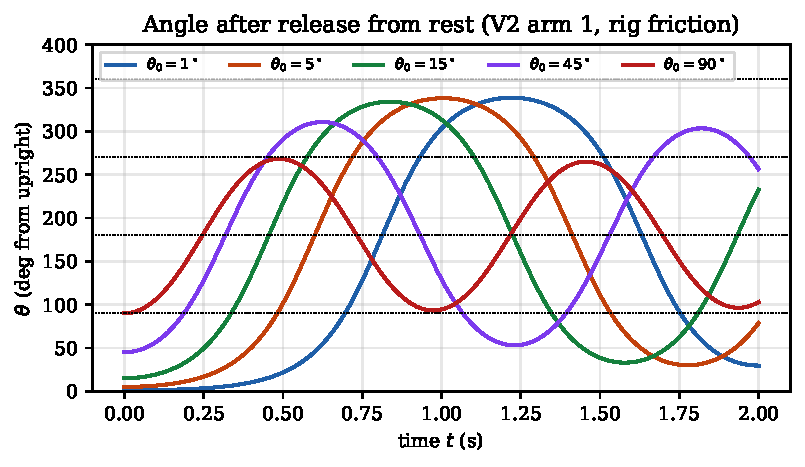
\includegraphics[width=0.9\linewidth]{figures/theta_vs_t.pdf}
\caption{$\theta(t)$ for several release angles. Small release angles spend most of the time near the top, then all fall at about the same rate.}
\end{figure}
\begin{figure}[h!]
\centering
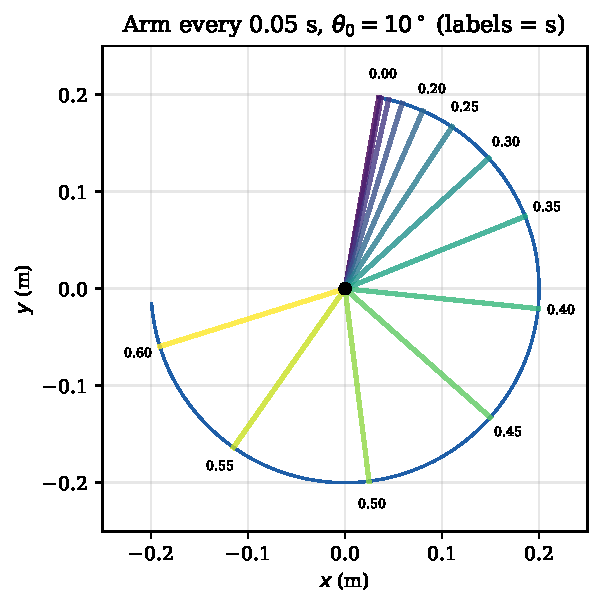
\includegraphics[width=0.48\linewidth]{figures/strobe.pdf}\hfill
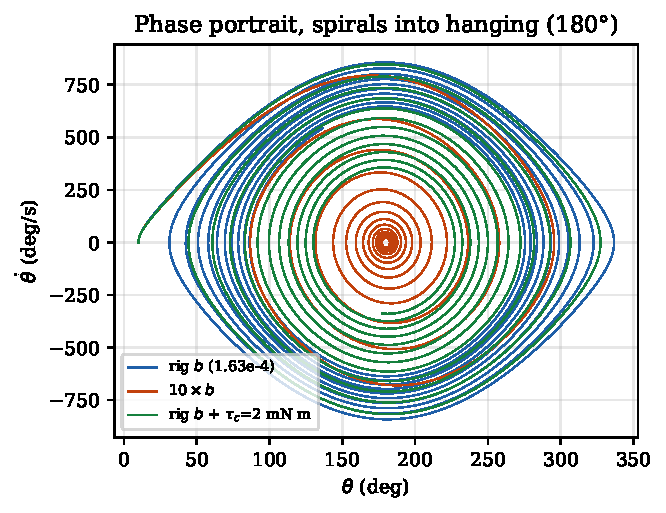
\includegraphics[width=0.48\linewidth]{figures/phase.pdf}
\caption{Left: arm drawn every 0.05\,s with the tip path (labels in seconds). Right: phase portrait for three friction cases; all spiral into hanging.}
\end{figure}
\begin{figure}[h!]
\centering
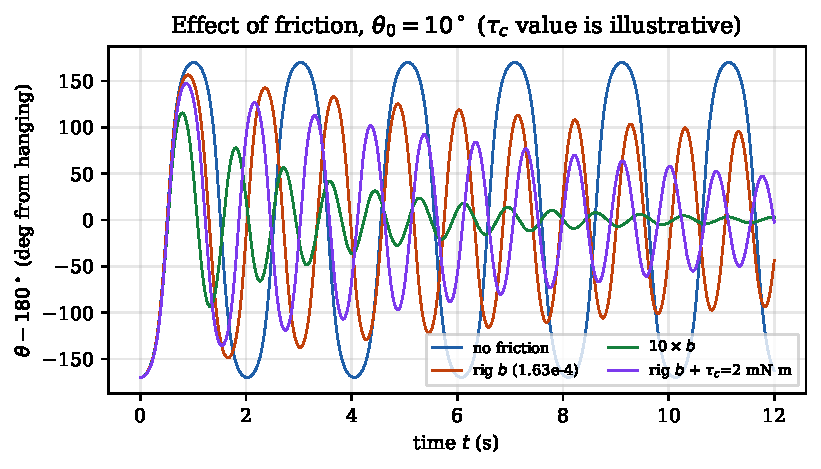
\includegraphics[width=0.9\linewidth]{figures/friction.pdf}
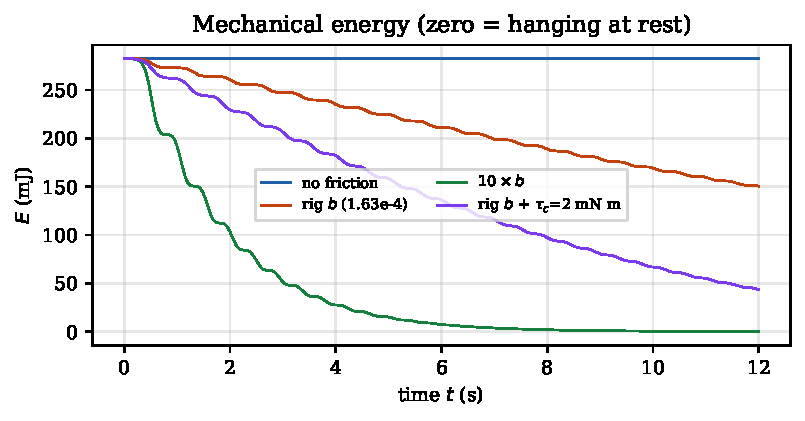
\includegraphics[width=0.9\linewidth]{figures/energy.pdf}
\caption{Effect of friction over 12\,s. Viscous friction gives an exponential decay; Coulomb friction a linear one, ending stuck. The $\tau_c=2$\,mN\,m case is illustrative, not measured.}
\end{figure}
\begin{figure}[h!]
\centering
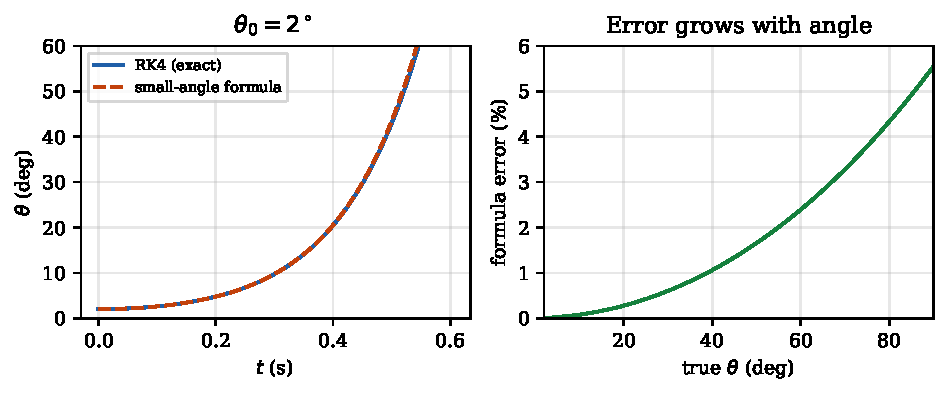
\includegraphics[width=0.9\linewidth]{figures/small_angle.pdf}
\caption{Small-angle formula \eqref{eq:lin} against the full nonlinear solution, $\theta_0=2^\circ$.}
\label{fig:small}
\end{figure}
\begin{figure}[h!]
\centering
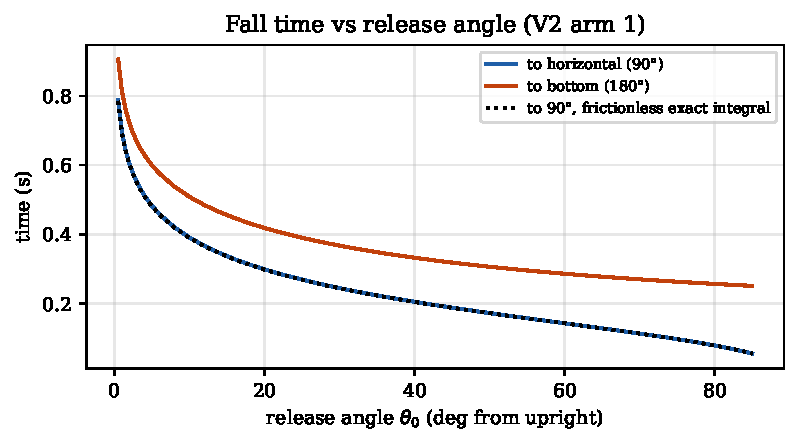
\includegraphics[width=0.9\linewidth]{figures/fall_time.pdf}
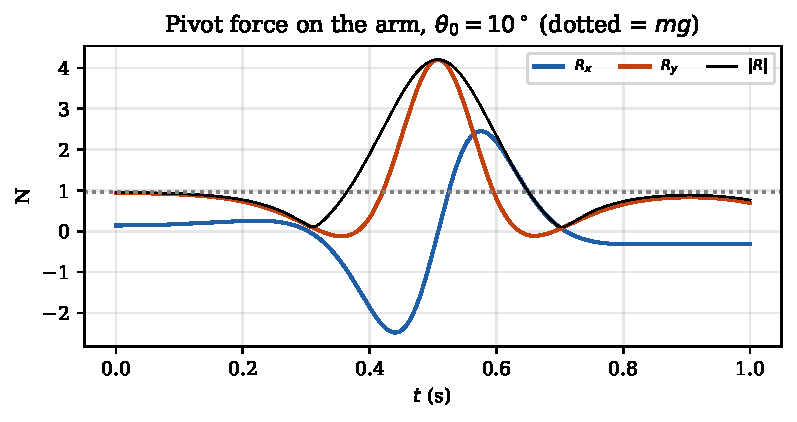
\includegraphics[width=0.9\linewidth]{figures/pivot_force.pdf}
\caption{Top: fall time to horizontal and to the bottom. Bottom: force on the pivot during the first second of a $10^\circ$ release.}
\end{figure}
\clearpage

%=====================================================================
\section{Measuring $b$ and $\tau_c$ on the rig}\label{sec:measure}
%=====================================================================
\begin{enumerate}
\item Lock the cart. Lift the arm to about $30^\circ$ from hanging and let go. Log $\theta$ at 100--200\,Hz until it stops.
\item Find the peak of each swing, $A_1, A_2, \dots$ (in rad, from hanging).
\item Plot $A_n$ against $n$. An exponential decay (straight line on a log scale, ratio $e^{-\pi\zeta/\sqrt{1-\zeta^2}}$ per half swing) means viscous friction. A straight-line decay of $2\tau_c/k$ per half swing, ending with the arm stuck slightly off hanging, means Coulomb friction. Real bearings usually show a mix: fast exponential decay at large swings, linear at the end.
\item Convert: $b=2\zeta\sqrt{Ik}$, $\tau_c=\tfrac12 k\,\Delta A_{half}$. For a mix, the most reliable route is to fit $b$ and $\tau_c$ directly by simulating \eqref{eq:ss} and minimizing the angle error, as the team already does for the cart model.
\item Check $I$ at the same time: the small-swing period gives $I=k/\omega_n^2=mgl_c(T_n/2\pi)^2$.
\end{enumerate}

\section*{Files}
In the project files, \texttt{FallingPendulum/}: this PDF and its \texttt{.tex}, \texttt{falling\_pendulum.py} (solver and CLI), \texttt{make\_figures.py}, \texttt{gen\_tables.py}, \texttt{figures/}, and \texttt{falling\_pendulum\_calculator.html} (the interactive table, also published as a web page).

\end{document}
